%descrizione del refinement e immagine sprint backlog
In questo sprint il refinement è iniziato ad essere più accurato, essendo la parte organizzativa volta quasi al termine. Il refinement è stato svolto incrementalmente e ha scomposto il design principale in più sotto-issue, ognuna corrispondente al model, alla view e al controller. Il raffinamento dei mockup è stato scomposto nel raffinamento di ogni schermata.  Infine, la userstory è stata scomposta nell avvio di una partita, nella creazione della pagina principale e nella creazione del meccanismo di domanda e risposta. 

Lo \href{https://github.com/orgs/ISIQuiz/projects/3/}{sprint backlog} risultante:

\begin{figure}[H]
    \centering
    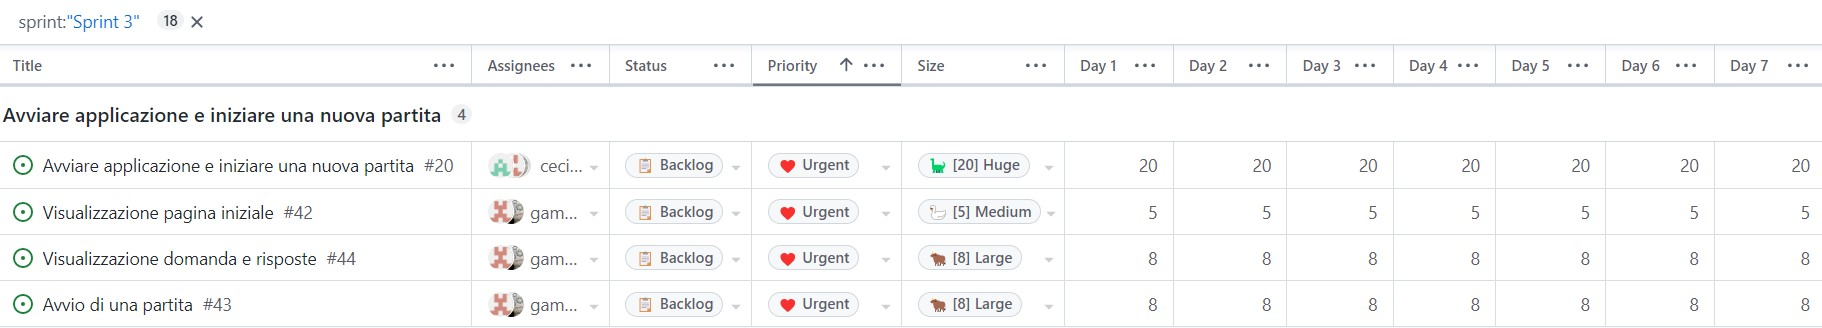
\includegraphics[width=\textwidth]{process/Img/Sprint3BL1.jpg}
    \label{fig:Sprint3BL1}
\end{figure}
\begin{figure}[H]
    \centering
    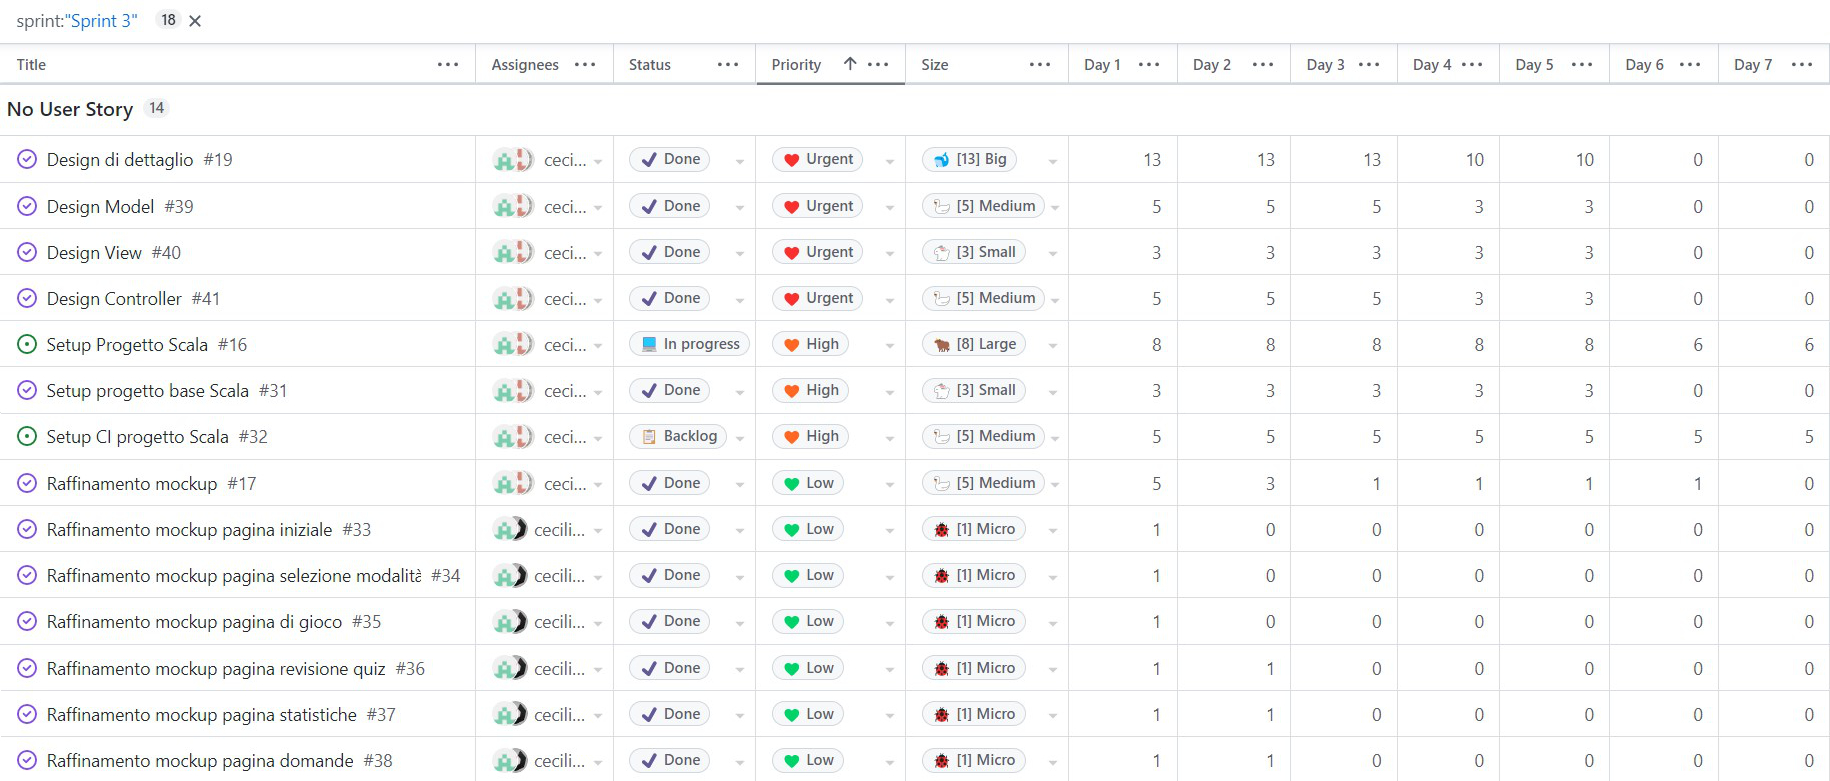
\includegraphics[width=\textwidth]{process/Img/Sprint3BL2.jpg}
    \label{fig:Sprint3BL2}
    \caption{Sprint 3 backlog}
\end{figure}
